\immediate\write18{tex braids.dtx}
\documentclass{ltxdoc}
\usepackage[T1]{fontenc}
\usepackage{lmodern}
\usepackage{morefloats}
\usepackage{tikz}
\usepackage{braids}
\usepackage[numbered]{hypdoc}
\definecolor{lstbgcolor}{rgb}{0.9,0.9,0.9} 
 
\usepackage{listings}
\lstloadlanguages{[LaTeX]TeX}
\lstset{breakatwhitespace=true,breaklines=true,language=TeX}
 
\usepackage{fancyvrb}

\newenvironment{example}
  {\VerbatimEnvironment
   \begin{VerbatimOut}{example.out}}
  {\end{VerbatimOut}
   \begin{center}
   \setlength{\parindent}{0pt}
   \fbox{\begin{minipage}{.9\linewidth}
     \lstset{breakatwhitespace=true,breaklines=true,language=TeX,basicstyle=\small}
     \lstinputlisting[]{example.out}
   \end{minipage}}

   \fbox{\begin{minipage}{.9\linewidth}
     \input{example.out}
   \end{minipage}}
\end{center}
}

\providecommand*{\url}{\texttt}
\GetFileInfo{braids.sty}

\title{The \textsf{braids} Package: Documentation}
\author{Andrew Stacey \\ \url{stacey@math.ntnu.no}}
\date{\fileversion~from \filedate}

\begin{document}

\maketitle

\begin{center}
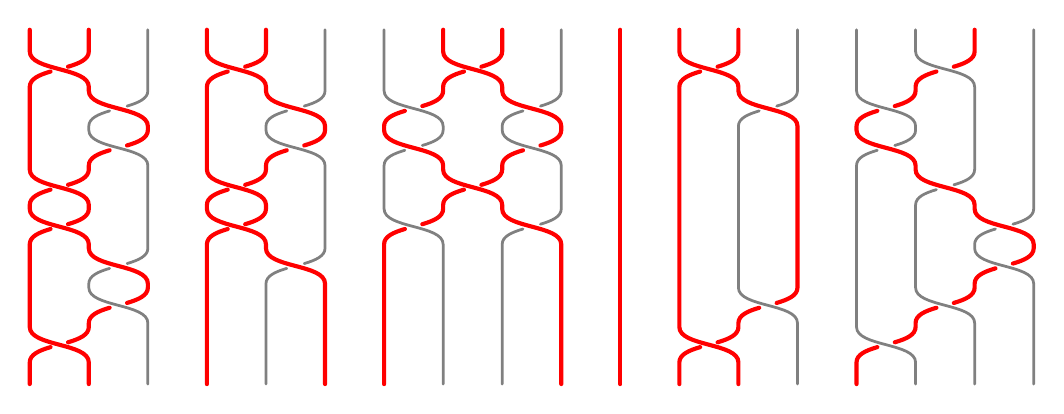
\begin{tikzpicture}
\braid[width=.75cm,height=.5cm,line width=1.5pt,red,line cap=round,style strands={3,6,7,10,14,15,16,18}{gray,line width=1pt}] s_1-s_4-s_8-s_{12}-s_{16} s_2-s_5-s_7-s_9-s_{13}-s_{15} s_2-s_5-s_7-s_9-s_{15} s_1-s_4-s_8-s_{16} s_1-s_4-s_7-s_9-s_{17} s_2-s_5-s_{17} s_2-s_{13}-s_{16} s_1-s_{12}-s_{15};
\end{tikzpicture}
\end{center}

\section{Introduction}

This is a package for drawing braid diagrams using PGF/TikZ.
An example follows.

\begin{example}
\begin{center}
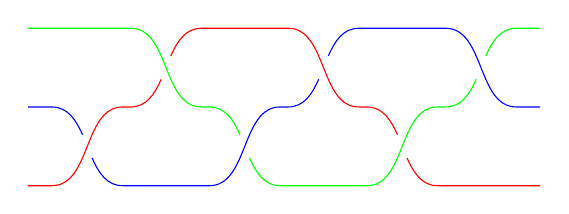
\begin{tikzpicture}
\braid[rotate=90,style strands={1}{red},style strands={2}{blue},style strands={3}{green}] s_1 s_2^{-1} s_1 s_2^{-1} s_1 s_2^{-1};
\end{tikzpicture}
\end{center}
\end{example}

\section{Usage}

\DescribeMacro{\braid}
A braid is specified by the command \Verb+\braid+.
The syntax for this command is as follows:

\Verb+\braid[style options] (name) at (coordinate) braid-word;+

\DescribeMacro{braid-word}
The \Verb+braid-word+ is an expression in the braid group, such as \Verb+s_1 s_2^{-1}+.
The generator labels are not significant.
The exponent can be \Verb+1+, \Verb+{-1}+, or missing (in which case it defaults to \Verb+1+, note also that the exponent is read as a \TeX-token so \Verb+{1}+ is also legal).
Certain other symbols are allowed in the \Verb+braid-word+ which control the rendering of the braid.
To get crossings to render at the same height, separate them with a hyphen (note: no check is made to ensure that the crossings can legally be put at the same height; \emph{caveat emptor}).
To draw a \emph{floor}, precede the braid element by a vertical line.
What happens then is that when the braid is rendered, the coordinates of the rectangle behind that crossing (wide enough to encompass all the strands) is passed to a command.
The intention is that this command draw something behind the braid.
The command is configurable by a key (see \ref{sec:styleopts}).

\DescribeMacro{name}
The (optional) \Verb+name+ acts a little like the \Verb+name+ of a TikZ node.
When it is specified, the routine that renders the braid also saves certain coordinates as if they were node anchors.
Specifically, \Verb+coordinate+ nodes are placed at the centre of the braid diagram and at the ends of each strand.
The centre has the label \Verb+name+, the strands are labelled \Verb+name-number-end+ and \Verb+name-rev-number-end+, where \Verb+name+ is the name given to the braid, \Verb+number+ is the number of the strand counting from the left, and \Verb+end+ is either \Verb+s+ for the start or \Verb+e+ for the end.
If the version with \Verb+rev+ is used then the numbers correspond to the \emph{final} positions of the braids.
The name can also be specified with the \Verb+name+ key.

\DescribeMacro{at}
The (optional) \Verb+at (coordinate)+ syntax positions the braid at the \Verb+coordinate+ in the current picture.
Due to the implementation, the coordinate has to be known at the start, but the width and height of the braid are only known at the end.
Therefore, the braid is positioned so that the start of the first strand is at \Verb+(coordinate)+.
This can also be specified using the \Verb+at+ key.

\DescribeMacro{style options}
The \Verb+style options+ set the style for the braid strands.
They can be grouped into three types: options that set up the main parameters for the braid, options that set the default style for the strands, and options that set up styles for individual strands.
The options are as follows.

\subsection{Style Options}
\label{sec:styleopts}

\DescribeMacro{number of strands} The key \Verb+number of strands+ sets the minimum number of strands for the braid.
The number of strands will grow according to the terms in the braid word so this merely sets a lower bound.
If not set, the number of strands will be determined by the terms in the braid word.

\DescribeMacro{height}
The key \Verb+height+ sets the height of the piece of the braid corresponding to an element in the group.

\DescribeMacro{width}
The key \Verb+width+ sets the separation of the strands in the braid.

\DescribeMacro{border height}
The key \Verb+border height+ adds a little extra length to the strands at the start and end of the braid.

\DescribeMacro{style strands}
The style of the strands are controlled by two types of option.
Style options that are set on the \Verb+\braid+ command are passed to every strand.
It is also possible to add style options to individual strands using the key \Verb+style strands+.
This takes two options, a comma-delimited list of strand numbers (which could be just a single number) and a list of options to be applied to that strand.
Thus, the syntax is \Verb+style strands={n,m,...}{options}+.
The strands are numbered by their starting position.
Not all of the standard TikZ style options are possible due to the way that the strands are constructed.
Basically, the options that are allowed are those that do not require changing the path or drawing it more than once.

\DescribeMacro{floor command}
When a floor is requested behind a crossing, the actual way to render it is determined by a command.
This key allows the user to define that command.
The argument to this key should be the code that should be executed for each floor.
To avoid the hassle of getting the number of hashes right, the command should take no arguments.
Rather, the coordinates of the rectangle are saved in to macros \Verb+\floorsx+, \Verb+\floorsy+, \Verb+\floorex+, \Verb+\floorey+ (these macros will expand to something like \Verb+10pt+) and the command should use these to position the drawing.
The default is to draw a line at the top and at the bottom of the rectangle.

\DescribeMacro{style floors}
\DescribeMacro{style all floors}
In the spirit of separating \emph{style} and \emph{content}, the style options for the floors can be specified separately to the command (of course, they could be built in to the command).
One advantage of this over building them in to the command is to allow them to be overridden for individual floors.
The \Verb+style all floors+ sets up options to be used for \emph{all} floors, whilst the \Verb+style floors={n,m,...}{options}+ sets up options to be used only for the listed floor.
Anything specified in the \Verb+floor command+ will take precedence over both of these.

Any other style options are passed to the underlying TikZ/PGF system and so may influence how the braid is drawn (but note that not all keys make sense due to the implementation).


\section{Example}

Here is a more detailed example.


\begin{example}
\begin{center}
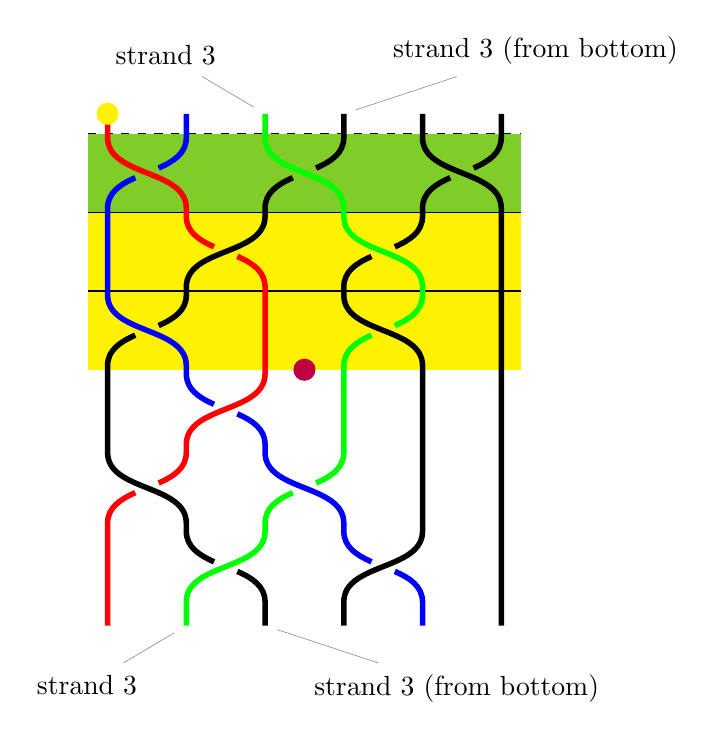
\begin{tikzpicture}
\braid[
  style all floors={fill=yellow},
  style floors={1}{dashed,fill=yellow!50!green},
  floor command={%
   \fill (\floorsx,\floorsy) rectangle (\floorex,\floorey);
   \draw (\floorsx,\floorsy) -- (\floorex,\floorsy);
  },
  line width=2pt,
  style strands={1}{red},
  style strands={2}{blue},
  style strands={3}{green}
] (braid) at (2,0) | s_1-s_3-s_5 | s_2^{-1}-s_4| s_1-s_4 s_2^{-1} s_1-s_3 s_2^{-1}-s_4^{-1};
\fill[yellow] (2,0) circle (4pt);
\fill[purple] (braid) circle (4pt);
\node[at=(braid-3-s),pin=north west:strand 3] {};
\node[at=(braid-3-e),pin=south west:strand 3] {};
\node[at=(braid-rev-3-s),pin=north east:strand 3 (from bottom)] {};
\node[at=(braid-rev-3-e),pin=south east:strand 3 (from bottom)] {};
\end{tikzpicture}
\end{center}
\end{example}
\end{document}

% Local Variables:
% tex-output-type: "pdf18"
% End:
